\documentclass[10.5pt]{article}
\usepackage[margin=0.95in]{geometry}
\IfFileExists{newtxtext.sty}{\usepackage{newtxtext,newtxmath}}{\usepackage{mathptmx}}
\IfFileExists{lmodern.sty}{\usepackage{lmodern}}{}
\usepackage[expansion=false]{microtype}
\usepackage{amsmath,amssymb}
\usepackage{booktabs,tabularx,multirow}
\usepackage{xcolor}
\usepackage[most]{tcolorbox}
\usepackage{enumitem}
\usepackage{tikz}
\usetikzlibrary{positioning,arrows.meta,fit,backgrounds,calc}
\usepackage{caption}
\usepackage[colorlinks=true,linkcolor=blue!50!black,citecolor=blue!50!black,urlcolor=blue!50!black]{hyperref}
\setlist{nosep,leftmargin=1.4em}
\captionsetup{font=small,labelfont=bf}
\definecolor{wm}{RGB}{38,84,124}
\definecolor{tg}{RGB}{173,98,40}
\definecolor{rt}{RGB}{46,125,90}
\newtcolorbox{note}[1][]{colback=gray!6,colframe=gray!55,boxrule=0.5pt,arc=1pt,left=6pt,right=6pt,top=4pt,bottom=4pt,#1}
\newcommand{\sg}{\operatorname{sg}}

\title{\textbf{GEMMA-WM: A Hierarchical Sequential JEPA World Model\\for Global Human-Mobility Modelling}\\[4pt]
\large Rationale, survey of world models, architecture, objectives, and pre-registered experimental plan}
\author{Technical design note for the GEMMA project\\(Global Embeddings for urban Mobility Modelling and Adaptation)\\[3pt]
Shiveswarran Ratneswaran, UMNI Lab, Purdue University --- October 2026}
\date{}

\begin{document}
\maketitle

\begin{note}
\textbf{Status and honesty note.} Every number in Section~\ref{sec:state} was measured in our own runs or taken from the
published Massive-STEPS benchmark~\cite{massivesteps}. \emph{No result for the new model in this note has been measured yet.}
Section~\ref{sec:plan} states pre-registered \emph{targets} and the criteria under which each hypothesis is rejected.
A paper must report whatever the runs produce, including negative ablations.
\end{note}

\section{Executive summary}
\begin{itemize}
\item \textbf{Goal.} Pretrain GEMMA once on large source cities so that next-POI recommendation in \emph{unseen} cities
(zero-, few- and full-shot) beats in-city supervised models (STHGCN~\cite{sthgcn}, GETNext~\cite{getnext},
LSTPM~\cite{lstpm}, Flashback~\cite{flashback}) and zero-shot LLM agents (LLM-Mob~\cite{llmmob}, LLM-ZS~\cite{llmzs},
LLM-Move~\cite{llmmove}).
\item \textbf{What we learned.} The original JEPA pretraining did not improve the backbone once the model was trained to
predict the next check-in on the source cities: a randomly initialised backbone reached the same Tokyo accuracy
(zero-shot 0.236 vs.\ 0.234). Gains so far come from user history and the realization stage, and almost none from
predicting places a user has never visited (``explore'' Acc@1 $\le 0.01$).
\item \textbf{Diagnosis.} The old JEPA had (i) a single latent target dominated by the POI-name embedding, (ii) a
one-step horizon, (iii) a predictor that never had to reason about \emph{decisions}, and (iv) its latent was not the
space in which retrieval happens, so pretrained knowledge had no direct path to the ranking.
\item \textbf{Proposal: HS-JEPA (Hierarchical Sequential JEPA).} One self-supervised world model that predicts, in
latent space and coarse-to-fine, the \emph{activity $\rightarrow$ primary category $\rightarrow$ secondary category
$\rightarrow$ place $\rightarrow$ return-or-explore} of the next $H$ check-ins, against \emph{hierarchical abstraction
targets} produced by an EMA target encoder. Retrieval is performed \emph{in the world model's latent space} by an exact
hierarchical return--explore mixture (Section~\ref{sec:retrieval}). Pretraining and retrieval become a single stage.
\item \textbf{Code.} \texttt{gemma/hsjepa.py} (model and losses), \texttt{gemma/hrem.py} (latent retrieval),
\texttt{scripts/run\_wm.sh} (pretraining, evaluation, ablations).
\end{itemize}

\section{Where we stand: measured results}\label{sec:state}
\begin{table}[h]
\centering\small
\caption{Tokyo (never used in pretraining), Massive-STEPS test split, ranking over all 2{,}982 city POIs.
``Revisit'' = target already in the user's history or prefix (52--53\% of cases); ``explore'' = new to the user.
GEMMA runs use the v5c realizer; zero-shot uses no Tokyo training data.}
\label{tab:tokyo}
\begin{tabular}{lcccccc}
\toprule
Model & Shot & Acc@1 & NDCG@5 & Revisit Acc@1 & Explore Acc@1 & Next-act.\ acc \\
\midrule
GEMMA v4 (old pipeline) & full & 0.107 & 0.170 & -- & -- & 0.364 \\
GEMMA v5c, JEPA backbone v4 & zero & 0.234 & 0.330 & 0.451 & 0.002 & 0.502 \\
GEMMA v5c, JEPA backbone v4 & full & 0.242 & 0.345 & 0.445 & 0.010 & 0.529 \\
GEMMA v5c, JEPA backbone v5 & zero & 0.218 & 0.313 & 0.421 & 0.000 & 0.487 \\
GEMMA v5c, \textbf{random backbone} & zero & 0.236 & 0.326 & 0.454 & 0.002 & 0.508 \\
GEMMA v5c, \textbf{random backbone} & full & 0.243 & 0.344 & 0.447 & 0.010 & 0.509 \\
\midrule
History-frequency heuristic (0 parameters) & -- & 0.175 & 0.296 & -- & 0.000 & -- \\
Activity heuristic (frequency + Markov) & -- & -- & -- & -- & -- & 0.530 \\
STHGCN~\cite{sthgcn} (published) & in-city & 0.250 & 0.350 & -- & -- & -- \\
LSTPM~\cite{lstpm} (published) & in-city & 0.225 & 0.315 & -- & -- & -- \\
\bottomrule
\end{tabular}
\end{table}

\paragraph{Source-city validation.} After pretraining on the six source cities, validation Acc@1 is 0.155 (v4 JEPA
init), 0.165 (v5 JEPA init) and 0.162 (random init). At initialisation the JEPA backbones start ahead (0.107/0.110 vs.\
0.087, next-activity 0.43 vs.\ 0.07), so JEPA learned useful structure, but the next-check-in objective on the same data
recovers it.

\paragraph{Zero-shot vs.\ LLMs.} Under the LLM protocol (200 users, 100 nearest POIs with the truth inserted), the
earlier 15-city run beat the best LLM-Move result in 6 of 9 held-out cities; Tokyo zero-shot 0.271--0.282 vs.\ 0.255.
Full-shot averaged 81\% of STHGCN and was above it only in Tokyo, within noise.

\paragraph{Benchmark facts that shape the design.}
\begin{itemize}
\item The current-trajectory prefix averages only 1.5--2.0 check-ins, so the user's history carries most of the signal.
\item 40--62\% of targets are already in the user's history; the rest are explorations.
\item The best LLM numbers rank roughly 101 candidates with the truth inserted, not the full vocabulary.
\end{itemize}

\section{Why a world model for global mobility}\label{sec:why}
\paragraph{Mobility as a partially observed decision process.} A user's day is a sequence of decisions
(\emph{what to do}, \emph{where}, \emph{return or try something new}) generated by a latent state: routine, purpose,
spatial anchors, time budget. A world model learns $p(s_{t+1}\mid s_{\le t})$ over such latent states. Prediction
\emph{in latent space} (JEPA~\cite{lecun2022path,ijepa,vjepa}) rather than over POI tokens has four properties that
matter for \emph{global} pretraining:
\begin{enumerate}
\item \textbf{Transfer.} Venue identities are city-specific (tens of thousands per city) and do not transfer. Latent
dynamics do: activity grammar, daily motifs~\cite{motifs}, distance decay, periodicity, exploration--return
balance~\cite{epr}.
\item \textbf{Ignoring the unpredictable.} Which of several equivalent caf\'es a user picks is close to irreducible
noise. A latent target can encode ``a caf\'e near the office at 9\,am'' without being penalised for the exact venue,
whereas a token-level generative objective spends capacity on that noise~\cite{lecun2022path}.
\item \textbf{Hierarchy matches behaviour.} Travel-behaviour theory models choice as nested decisions (activity, then
destination; nested logit and activity-based models~\cite{benakiva,bowman}). A hierarchical latent predictor is the
neural, self-supervised counterpart of that nesting.
\item \textbf{Planning and counterfactuals.} A latent world model can roll forward several steps (next $H$ check-ins)
and score hypothetical futures, which pure retrieval models cannot.
\end{enumerate}

\paragraph{Why our first JEPA did not help, and what changes.}
\begin{center}\small
\begin{tabularx}{\linewidth}{>{\raggedright\arraybackslash}p{4.7cm}X}
\toprule
Failure in GEMMA v4/v5 & HS-JEPA remedy \\
\midrule
One latent target per check-in, dominated by the LLM name embedding & Four hierarchical abstraction targets (activity, primary, secondary, place) from the same EMA target encoder \\
One-step horizon & Multi-horizon prediction of the next $H{=}3$ check-ins (block-causal) \\
No decision variable in the latent & Explicit return-or-explore query, read out as an activity-conditioned gate \\
Pooled-context predictor & Cross-attention predictor over all context states \\
Retrieval in a separately learned space & Retrieval reads the predicted latents directly (pointer into latent memory, latent--POI matching) \\
Two stages (JEPA, then next-place) & One stage: JEPA losses and the retrieval likelihood trained jointly from step 0 \\
\bottomrule
\end{tabularx}
\end{center}

\section{Survey: world models and their fit for mobility}\label{sec:survey}
\begin{table}[h]
\centering\small
\caption{World-model families. ``Fit'' is our judgement for city-agnostic check-in modelling with huge, city-specific
item vocabularies and no actions.}
\begin{tabularx}{\linewidth}{>{\raggedright\arraybackslash}p{3.0cm}>{\raggedright\arraybackslash}p{3.4cm}>{\raggedright\arraybackslash}p{3.3cm}X}
\toprule
Family & Examples & Predicts & Fit for global mobility \\
\midrule
Latent RL world models (RSSM) & World Models~\cite{worldmodels}, PlaNet~\cite{planet}, DreamerV3~\cite{dreamerv3} & Stochastic latent + reconstruction of observations & Good latent dynamics, but the reconstruction loss forces modelling venue identity; no actions here. Option: stochastic latent as an ablation. \\
Value-equivalent models & MuZero~\cite{muzero} & Reward/value/policy-relevant latents & Needs rewards and actions; not applicable without a planning task. \\
Latent MPC models & TD-MPC2~\cite{tdmpc2} & Latent dynamics + value, no reconstruction & Elegant latent-only training, but action-centric. \\
Token autoregressive world models & IRIS~\cite{iris}, Genie~\cite{genie}, GAIA-1~\cite{gaia1}, Cosmos~\cite{cosmos} & Discrete tokens of future observations & Applicable via semantic IDs~\cite{tiger}; spends capacity on identity noise; we keep it only as an auxiliary decoder. \\
Diffusion world models & DIAMOND~\cite{diamond} & Denoised future observations & Strong for pixels; costly and identity-centric for POIs. \\
\textbf{Joint-embedding predictive (JEPA)} & I-JEPA~\cite{ijepa}, V-JEPA~\cite{vjepa}, V-JEPA~2~\cite{vjepa2}, MC-JEPA~\cite{mcjepa}, LeJEPA~\cite{lejepa}; H-JEPA (concept)~\cite{lecun2022path} & Latent of masked/future content & \textbf{Best fit}: latent targets transfer across cities; V-JEPA~2 shows latent predictors can be action-conditioned and used for planning. \\
Frozen-feature latent dynamics & DINO-WM~\cite{dinowm} & Dynamics on pretrained features & Analogue: dynamics over frozen LLM POI embeddings; weaker than learning the encoder. \\
\midrule
Trajectory JEPAs & T-JEPA~\cite{tjepa}, HiT-JEPA~\cite{hitjepa} & Latents of masked trajectory parts & Closest prior work: built for \emph{trajectory similarity}. HiT-JEPA's hierarchy is spatial granularity (point / intermediate / whole), not semantic decisions. \\
LLM mobility agents & LLM-Mob~\cite{llmmob}, LLM-ZS~\cite{llmzs}, LLM-Move~\cite{llmmove} & Next place via prompting & Zero-shot, but billion-parameter and evaluated on small candidate lists. \\
\bottomrule
\end{tabularx}
\end{table}

\paragraph{Choice.} We keep the JEPA family as the world-model core. We add (a) hierarchical, decision-aligned latent
targets, (b) multi-horizon sequential prediction, and (c) latent-space retrieval. The semantic-ID autoregressive head
stays as an auxiliary generative decoder, and a stochastic-latent RSSM variant is listed as future work.

\paragraph{Novelty against prior work (to be checked in the related-work pass).} H-JEPA is a conceptual proposal in
\cite{lecun2022path}. HiT-JEPA~\cite{hitjepa} is hierarchical over spatial scale for trajectory similarity. To our
knowledge, HS-JEPA is the first JEPA whose hierarchy follows the \emph{semantic decision hierarchy}
(activity $\rightarrow$ category $\rightarrow$ place $\rightarrow$ return/explore) with abstraction-level targets, and
the first to perform next-POI retrieval inside the JEPA latent space across cities.

\section{HS-JEPA: architecture}\label{sec:arch}
\begin{figure}[t]
\centering
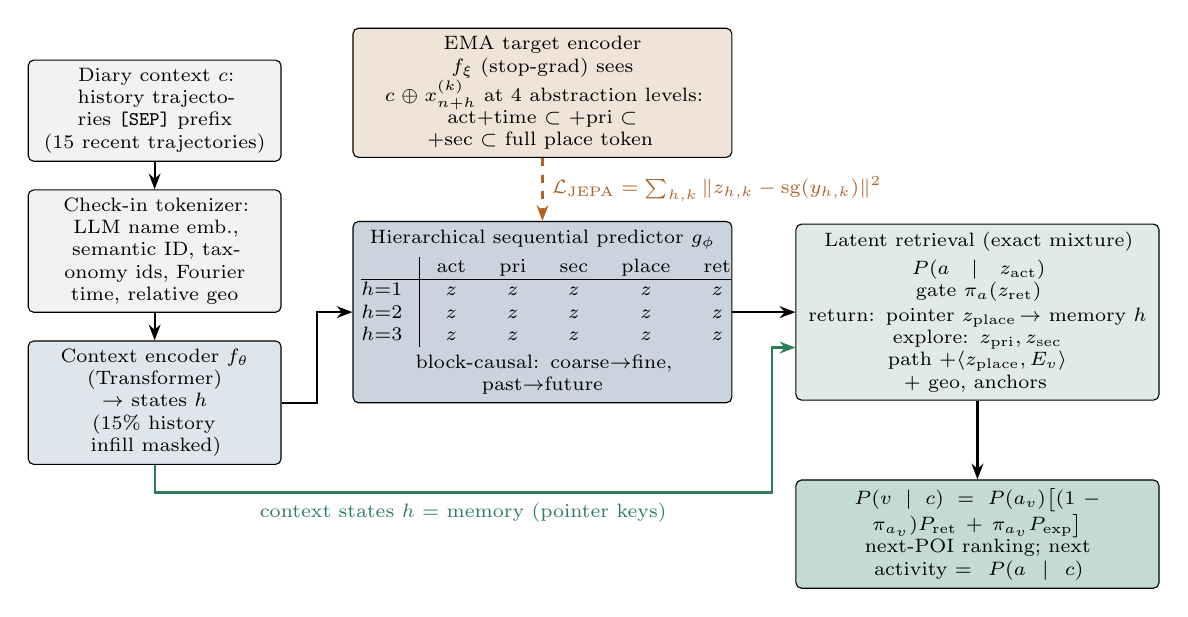
\begin{tikzpicture}[font=\scriptsize,
  box/.style={draw,rounded corners=2pt,align=center,minimum height=0.75cm,inner sep=3pt},
  arr/.style={-{Stealth[length=2mm]},thick},
  darr/.style={-{Stealth[length=2mm]},thick,dashed}]
\node[box,fill=gray!10,text width=3.0cm] (in) {Diary context $c$:\\ history trajectories \texttt{[SEP]} prefix\\(15 recent trajectories)};
\node[box,fill=gray!10,text width=3.0cm,below=0.35cm of in] (tok) {Check-in tokenizer: LLM name emb., semantic ID, taxonomy ids, Fourier time, relative geo};
\node[box,fill=wm!15,text width=3.0cm,below=0.35cm of tok] (enc) {Context encoder $f_\theta$\\(Transformer) $\rightarrow$ states $h$\\(15\% history infill masked)};
\draw[arr] (in) -- (tok); \draw[arr] (tok) -- (enc);

\node[box,fill=wm!25,text width=4.6cm,right=0.9cm of enc,yshift=1.15cm] (pred) {Hierarchical sequential predictor $g_\phi$\\[2pt]
\begin{tabular}{@{}c|ccccc@{}}
 & act & pri & sec & place & ret\\\hline
$h{=}1$ & $z$ & $z$ & $z$ & $z$ & $z$\\
$h{=}2$ & $z$ & $z$ & $z$ & $z$ & $z$\\
$h{=}3$ & $z$ & $z$ & $z$ & $z$ & $z$\\
\end{tabular}\\[2pt] block-causal: coarse$\rightarrow$fine, past$\rightarrow$future};
\draw[arr] (enc.east) -- ++(0.45,0) |- (pred.west);

\node[box,fill=tg!18,text width=4.6cm,above=0.8cm of pred] (tgt) {EMA target encoder $f_\xi$ (stop-grad) sees\\
$c\oplus x^{(k)}_{n+h}$ at 4 abstraction levels:\\ act+time $\subset$ +pri $\subset$ +sec $\subset$ full place token};
\draw[darr,tg] (tgt.south) -- node[right,xshift=2pt,fill=white,inner sep=1pt]{$\mathcal{L}_{\mathrm{JEPA}}=\sum_{h,k}\|z_{h,k}-\sg(y_{h,k})\|^2$} (pred.north);

\node[box,fill=rt!15,text width=4.4cm,right=0.8cm of pred] (ret) {Latent retrieval (exact mixture)\\[2pt]
$P(a\mid z_{\mathrm{act}})$ \\ gate $\pi_a(z_{\mathrm{ret}})$ \\[1pt]
return: pointer $z_{\mathrm{place}}\!\to$ memory $h$\\
explore: $z_{\mathrm{pri}},z_{\mathrm{sec}}$ path $+\langle z_{\mathrm{place}},E_v\rangle$\\$+$ geo, anchors};
\draw[arr] (pred.east) -- (ret.west);
\draw[arr,rt] (enc.south) -- ++(0,-0.35) coordinate (ma) -- (ma -| {$(ret.west)+(-0.3,0)$}) node[pos=0.5,below]{context states $h$ = memory (pointer keys)} coordinate (mb) |- ($(ret.west)+(0,-0.45)$);

\node[box,fill=rt!28,text width=4.4cm,below=0.45cm of ret,yshift=-0.55cm] (out) {$P(v\mid c)=P(a_v)\big[(1-\pi_{a_v})P_{\mathrm{ret}}+\pi_{a_v}P_{\mathrm{exp}}\big]$\\ next-POI ranking; next activity $=P(a\mid c)$};
\draw[arr] (ret) -- (out);
\end{tikzpicture}
\caption{GEMMA-WM. One self-supervised model: context encoder, hierarchical sequential predictor trained against
hierarchical abstraction targets (JEPA), and retrieval performed directly on the predicted latents.}
\label{fig:arch}
\end{figure}

\paragraph{Tokens.} Each check-in token combines the LLM embedding of ``category : name'', the 4-level semantic ID
(RQ-VAE), activity/primary/secondary ids from the Foursquare taxonomy, multi-scale Fourier time (hour, weekday,
month), and relative motion (log-distance, bearing). All features are city-agnostic.

\paragraph{Context encoder.} The online encoder $f_\theta$ (4-layer Transformer, $d{=}256$) reads the diary
$c=[\text{trail}_1]\,\texttt{SEP}\cdots\texttt{SEP}\,[\text{prefix}]$ and outputs states $h\in\mathbb{R}^{L\times d}$.

\paragraph{Hierarchical sequential predictor.} For horizons $h=1..H$ and levels
$k\in\{\text{act},\text{pri},\text{sec},\text{place},\text{ret}\}$, a query
$q_{h,k}=[\textsc{mask}]+\mathrm{pos}(n{+}h)+e^{\mathrm{lvl}}_k+e^{\mathrm{hor}}_h+\bar h$ cross-attends to $h$. Under a
block-causal mask, $q_{h,k}$ may attend to $q_{h',k'}$ if $h'<h$, or if $h'=h$ and $k'\le k$:
\begin{equation}
z_{h,k}=g_\phi\big(q_{h,k}\mid h;\ z_{<h,\cdot},\,z_{h,<k}\big).
\end{equation}
The place latent is therefore predicted \emph{conditioned on the predicted activity and category latents}, the
sequential hierarchy, and step $h{+}1$ is conditioned on the predicted step $h$, a latent rollout.

\paragraph{Hierarchical abstraction targets.} The EMA target encoder $f_\xi$ ($\xi\leftarrow\tau\xi+(1-\tau)\theta$)
sees the full context plus the true future check-in at four levels of detail: $x^{(\text{act})}$ = activity id + time;
$x^{(\text{pri})}$ = + primary id; $x^{(\text{sec})}$ = + secondary id; $x^{(\text{place})}$ = the full token:
\begin{equation}
y_{h,k}=\mathrm{LN}\big(f_\xi(c\oplus x^{(k)}_{n+h})\big)_{n+h},\qquad
\mathcal{L}_{\mathrm{JEPA}}=\frac{1}{4}\sum_{k\le\text{place}}\frac{1}{|\mathcal V|}\sum_{h\in\mathcal V}\|z_{h,k}-\sg(y_{h,k})\|_2^2 .
\end{equation}
Each level must encode exactly the information of its abstraction, so the latent space becomes hierarchical by
construction rather than by hope.

\section{Self-supervised objectives and masking}\label{sec:ssl}
All targets come from the check-in stream itself; no human labels are used.
\begin{align}
\mathcal{L}=\underbrace{-\log P(v^\star\mid c)}_{\text{latent retrieval}}
+0.3\,\underbrace{\mathrm{BCE}(\pi_{a^\star},\mathbb 1[v^\star\text{ new}])}_{\text{return/explore}}
+\lambda_J\mathcal{L}_{\mathrm{JEPA}}+\lambda_I\mathcal{L}_{\mathrm{infill}}
+\lambda_P\!\!\sum_{h,\ell\in\{a,p,s\}}\!\!\mathrm{CE}(\ell_{h})+\lambda_R\,\mathrm{VICReg}(h)
\end{align}
Defaults: $\lambda_J{=}1$, $\lambda_I{=}0.5$, $\lambda_P{=}0.5$, $\lambda_R{=}0.1$, $H{=}3$; SIGReg~\cite{lejepa} is an option
in place of VICReg~\cite{vicreg}. A light semantic-ID decoder loss keeps the generative head~\cite{tiger} trained on
$z_{1,\mathrm{place}}$.

\paragraph{Masking strategy.} The masking defines what the world model must predict, so it should rehearse the
downstream question without making it trivial:
\begin{center}\small
\begin{tabularx}{\linewidth}{>{\raggedright\arraybackslash}p{3.3cm}X>{\raggedright\arraybackslash}p{2.6cm}}
\toprule
Strategy & What it teaches & Used? \\
\midrule
Future block (next $H$) & Dynamics and multi-step rollout; exactly the downstream query & \textbf{Yes} (main view) \\
Hierarchical abstraction & Coarse-to-fine decision structure; transferable activity/category grammar & \textbf{Yes} (targets) \\
History infill (15\%) & Representation of the user's routine and memory (bidirectional) & \textbf{Yes} (second view) \\
Random span / activity block (v4) & Generic interpolation; leaks future context into the input & Ablation only \\
Whole-trajectory masking & Day-level routine (motif) prediction & Future work \\
\bottomrule
\end{tabularx}
\end{center}

\section{World-model retrieval}\label{sec:retrieval}
Retrieval reads the predicted latents of step $h{=}1$:
\begin{equation}
P(v\mid c)=P(a_v\mid c)\Big[(1-\pi_{a_v}(c))\,P_{\mathrm{ret}}(v\mid c,a_v)+\pi_{a_v}(c)\,P_{\mathrm{exp}}(v\mid c,a_v)\Big].
\end{equation}
\begin{itemize}
\item \textbf{Activity} $P(a\mid c)$: probe on $z_{1,\mathrm{act}}$ plus the user's activity profile and activity
transitions. It therefore contains the heuristic signals, and the next-activity prediction is this distribution.
\item \textbf{Gate} $\pi_a(c)=\sigma\big(w^\top z_{1,\mathrm{ret}}+\beta_1\operatorname{logit}\nu_{u,a}+\beta_2\log
S_u+\dots\big)$. Here $\nu_{u,a}$ is the user's first-visit rate in activity $a$, and $\beta_2\log S_u$ is the EPR
law~\cite{epr} $P(\text{explore})\propto S_u^{-\gamma}$ in logit form, so the learned $\beta_2$ is an estimate of
$-\gamma$.
\item \textbf{Return} $P_{\mathrm{ret}}$: softmax over visited POIs of activity $a$. It combines a latent pointer
$\langle W_q z_{1,\mathrm{place}},W_k h_j\rangle$ (the world model reading its memory) with recency, time-of-day and
weekday affinity (as in Flashback~\cite{flashback}), personal transitions and distance.
\item \textbf{Explore} $P_{\mathrm{exp}}$: softmax over unvisited POIs of activity $a$. It combines the predicted
category path $\log p(p_v\mid z_{\mathrm{pri}})+\log p(s_v\mid z_{\mathrm{sec}})$, the latent match
$\tau\cos(z_{1,\mathrm{place}},E_v)$ with the POI's semantic-ID/LLM embedding $E_v$, distance from the last check-in,
and distance to the user's anchors. Target-city transition, popularity and time-of-day statistics are added only in
few/full-shot.
\end{itemize}
The mixture is exactly normalised (verified $\sum_v P(v\mid c)=1$). Nothing is pruned, so there is no recall ceiling,
and new places can win when the gate says the user is exploring. This explicitly targets the explore Acc@1
$\approx 0$ failure in Table~\ref{tab:tokyo}.

\section{Experimental plan and pre-registered hypotheses}\label{sec:plan}
\paragraph{Protocol.}
\begin{itemize}
\item Massive-STEPS splits; ranking over all city POIs.
\item The LLM protocol is reported separately: 200 users, 5 seeds, three candidate sets.
\item 9 held-out cities for true zero-shot (or a 3-fold city split so all 15 are held out); 3 seeds.
\item Baselines: STHGCN, GETNext, LSTPM, Flashback (published, and re-run on three cities); LLM-Mob, LLM-ZS,
LLM-Move; history and activity heuristics; and the same architecture trained only on the target city.
\end{itemize}

\begin{table}[h]
\centering\small
\caption{Hypotheses, measurements and rejection criteria. ``Target'' values are goals, not results.}
\begin{tabularx}{\linewidth}{>{\raggedright\arraybackslash}p{4.3cm}>{\raggedright\arraybackslash}p{3.2cm}X}
\toprule
Hypothesis & Measured by & Target / rejected if \\
\midrule
H1: HS-JEPA pretraining helps transfer & zero-shot and 5\% few-shot vs.\ the same model with $\lambda_J{=}\lambda_I{=}0$ & Target $\ge$+0.02 Acc@1 on held-out cities; rejected if the gap is within one SE \\
H2: the hierarchy matters & full model vs.\ \texttt{--wm\_flat} & Target: higher explore Acc@5 and next-activity; rejected if equal \\
H3: multi-horizon helps & $H{=}3$ vs.\ $H{=}1$ & Rejected if equal within one SE \\
H4: global pretraining beats in-city learning & GEMMA vs.\ the same model trained only on the target & Target: largest gain in small cities; rejected if no gain \\
H5: the mixture unlocks exploration & explore Acc@1/@5 vs.\ v5c (0.010 / 0.051 in Tokyo) & Target explore Acc@1 $\ge 0.03$ \\
H6: next activity & vs.\ frequency+Markov heuristic (0.530 in Tokyo) & Target $\ge$ heuristic in every city \\
H7: overall & Acc@1/NDCG@5 vs.\ STHGCN and LLM-Move (matched protocols) & Target: above STHGCN in a majority of cities and above LLM-Move in all held-out cities, with 3-seed CIs \\
H8: the gate recovers mobility law & learned $\beta_2$ across cities & Consistent negative $\beta_2$ ($\gamma>0$) \\
\bottomrule
\end{tabularx}
\end{table}

\paragraph{Scaling.} The strongest evidence for a foundation model is a curve: held-out zero-shot accuracy versus
pretraining data, from 1 to 6 source cities and then to Semantic-Trails scale (STD 2013/2018 cover thousands of
cities~\cite{std}; the 15 benchmark cities must be excluded).

\section{Risks and honest limitations}
\begin{itemize}
\item \textbf{The JEPA terms may still add nothing when next-place data is abundant.} H1 tests exactly this; if
rejected, the paper reports it and positions HS-JEPA's value at small data or out-of-distribution cities, where the
measured initialisation advantage (Section~\ref{sec:state}) suggests it may matter.
\item \textbf{Compute.} Four target-encoder passes per step, about $2\times$ the cost of the v5 realizer; pretraining
takes several hours per run on one 24\,GB GPU.
\item \textbf{Protocol dependence.} LLM baselines are taken from published tables. Their candidate construction is
inferred, so we report all three variants and plan to re-run LLM-Move.
\item \textbf{Non-causal history} in the random benchmark split is shared with all baselines; we report a causal-history
ablation.
\end{itemize}

\section{Implementation map}
\begin{center}\small
\begin{tabularx}{\linewidth}{lX}
\toprule
File & Content \\
\midrule
\texttt{gemma/hsjepa.py} & \texttt{HPredictor} (block-causal hierarchical predictor), \texttt{WMHead}, \texttt{wm\_forward} (online + 4 target passes, infill, probes, regulariser) \\
\texttt{gemma/hrem.py} & \texttt{hrem\_mixture}: exact activity $\rightarrow$ gate $\rightarrow$ return/explore retrieval used by the world model \\
\texttt{gemma/realize.py} & City index, user-history evidence, training loop (EMA hook, AMP, mid-epoch validation), evaluation \\
\texttt{scripts/train\_realizer\_source.py} & Source-city pretraining (\texttt{--retriever wm}) \\
\texttt{scripts/run\_downstream.py} & Zero/few/full evaluation, both protocols \\
\texttt{scripts/run\_wm.sh} & Pretraining from scratch, Tokyo evaluation, old-JEPA-initialised variant, ablations (\texttt{ABLATIONS=1}), 15 cities (\texttt{ALL\_CITIES=1}) \\
\bottomrule
\end{tabularx}
\end{center}

\begin{thebibliography}{99}\small
\bibitem{massivesteps} W.~Wongso, H.~Xue, F.~D.~Salim. Massive-STEPS: Massive Semantic Trajectories for Understanding POI Check-ins -- Dataset and Benchmarks. arXiv:2505.11239, 2025.
\bibitem{std} D.~Monti et al. Semantic Trails of City Explorations: How Do We Live a City. arXiv:1812.04367, 2018.
\bibitem{lecun2022path} Y.~LeCun. A Path Towards Autonomous Machine Intelligence. OpenReview, 2022.
\bibitem{ijepa} M.~Assran et al. Self-Supervised Learning from Images with a Joint-Embedding Predictive Architecture. CVPR 2023 (arXiv:2301.08243).
\bibitem{vjepa} A.~Bardes et al. Revisiting Feature Prediction for Learning Visual Representations from Video (V-JEPA). arXiv:2404.08471, 2024.
\bibitem{vjepa2} M.~Assran et al. V-JEPA 2: Self-Supervised Video Models Enable Understanding, Prediction and Planning. arXiv:2506.09985, 2025.
\bibitem{mcjepa} A.~Bardes, J.~Ponce, Y.~LeCun. MC-JEPA: A Joint-Embedding Predictive Architecture for Self-Supervised Learning of Motion and Content Features. arXiv:2307.12698, 2023.
\bibitem{lejepa} R.~Balestriero, Y.~LeCun. LeJEPA: Provable and Scalable Self-Supervised Learning Without the Heuristics. arXiv:2511.08544, 2025.
\bibitem{vicreg} A.~Bardes, J.~Ponce, Y.~LeCun. VICReg: Variance-Invariance-Covariance Regularization for Self-Supervised Learning. ICLR 2022.
\bibitem{worldmodels} D.~Ha, J.~Schmidhuber. World Models. arXiv:1803.10122, 2018.
\bibitem{planet} D.~Hafner et al. Learning Latent Dynamics for Planning from Pixels (PlaNet). ICML 2019.
\bibitem{dreamerv3} D.~Hafner et al. Mastering Diverse Domains through World Models (DreamerV3). arXiv:2301.04104, 2023.
\bibitem{muzero} J.~Schrittwieser et al. Mastering Atari, Go, Chess and Shogi by Planning with a Learned Model. Nature 2020.
\bibitem{tdmpc2} N.~Hansen, H.~Su, X.~Wang. TD-MPC2: Scalable, Robust World Models for Continuous Control. ICLR 2024.
\bibitem{iris} V.~Micheli, E.~Alonso, F.~Fleuret. Transformers are Sample-Efficient World Models (IRIS). ICLR 2023.
\bibitem{genie} J.~Bruce et al. Genie: Generative Interactive Environments. ICML 2024.
\bibitem{gaia1} A.~Hu et al. GAIA-1: A Generative World Model for Autonomous Driving. arXiv:2309.17080, 2023.
\bibitem{cosmos} NVIDIA. Cosmos World Foundation Model Platform for Physical AI. arXiv:2501.03575, 2025.
\bibitem{diamond} E.~Alonso et al. Diffusion for World Modeling: Visual Details Matter in Atari (DIAMOND). NeurIPS 2024.
\bibitem{dinowm} G.~Zhou et al. DINO-WM: World Models on Pre-trained Visual Features enable Zero-shot Planning. arXiv:2411.04983, 2024.
\bibitem{tjepa} L.~Li et al. T-JEPA: A Joint-Embedding Predictive Architecture for Trajectory Similarity Computation. arXiv:2406.12913, 2024.
\bibitem{hitjepa} L.~Li, H.~Xue, S.~Ao, Y.~Song, F.~Salim. HiT-JEPA: A Hierarchical Self-supervised Trajectory Embedding Framework for Similarity Computation. arXiv:2507.00028, 2025.
\bibitem{tiger} S.~Rajput et al. Recommender Systems with Generative Retrieval (TIGER). NeurIPS 2023.
\bibitem{sthgcn} X.~Yan et al. Spatio-Temporal Hypergraph Learning for Next POI Recommendation. SIGIR 2023.
\bibitem{getnext} S.~Yang, J.~Liu, K.~Zhao. GETNext: Trajectory Flow Map Enhanced Transformer for Next POI Recommendation. SIGIR 2022.
\bibitem{lstpm} K.~Sun et al. Where to Go Next: Modeling Long- and Short-Term User Preferences for Point-of-Interest Recommendation. AAAI 2020.
\bibitem{flashback} D.~Yang et al. Location Prediction over Sparse User Mobility Traces Using RNNs: Flashback in Hidden States! IJCAI 2020.
\bibitem{llmmob} X.~Wang et al. Where Would I Go Next? Large Language Models as Human Mobility Predictors. arXiv:2308.15197, 2023.
\bibitem{llmzs} C.~Beneduce, B.~Lepri, M.~Luca. Large Language Models are Zero-Shot Next Location Predictors. arXiv:2405.20962, 2024.
\bibitem{llmmove} S.~Feng et al. Where to Move Next: Zero-shot Generalization of LLMs for Next POI Recommendation. 2024.
\bibitem{epr} C.~Song, T.~Koren, P.~Wang, A.-L.~Barab\'asi. Modelling the Scaling Properties of Human Mobility. Nature Physics 6, 2010.
\bibitem{motifs} C.~M.~Schneider et al. Unravelling Daily Human Mobility Motifs. J.\ R.\ Soc.\ Interface 10, 2013.
\bibitem{benakiva} M.~Ben-Akiva, S.~R.~Lerman. Discrete Choice Analysis: Theory and Application to Travel Demand. MIT Press, 1985.
\bibitem{bowman} J.~L.~Bowman, M.~E.~Ben-Akiva. Activity-based Disaggregate Travel Demand Model System with Activity Schedules. Transportation Research Part A 35(1), 2001.
\end{thebibliography}
\end{document}
